\documentclass[a4paper,11pt]{report}

\usepackage{amsmath,amsfonts,amssymb}
\usepackage{graphics}
\usepackage{graphicx}
\usepackage{booktabs}
\usepackage{tabularx}
\usepackage{array}
\usepackage{icomma}
\usepackage{tikz, ifthen}
\usetikzlibrary{arrows,shapes,backgrounds,patterns,decorations.pathreplacing,decorations.pathmorphing}

% <Temporary FHSST definitions>
\def\Definition#1#2{\paragraph{Definition:} #1 --- #2}

\def\Identity#1#2{\paragraph{Identity:} #1 --- #2}

\newenvironment{wex}[3]%
{\rule{\linewidth}{0.5mm}
\textbf{Worked example:} #1

\textbf{Question:} #2

\textbf{Solution:} #3}%
{\rule{\linewidth}{0.5mm}}

\newcommand{\westep}[1]{\paragraph{Step:} #1}

\newenvironment{exercises}[1]%
{\rule{\linewidth}{0.5mm}
\textbf{Exercises:} #1\\}%
{\rule{\linewidth}{0.5mm}}

\newenvironment{eocexercises}[1]%
{\section{End of chapter exercises: #1}}%
{}
% </Temporary FHSST definitions>

% <Temporary spacing changes>
\setlength\parindent{0pt}
\setlength\parskip{0.5\baselineskip}
\setlength\textwidth{15cm}
\setlength\textheight{23cm}
\setlength\oddsidemargin{0.5cm}
\setlength\topmargin{0cm}
% </Temporary spacing changes>

\begin{document}
\chapter{Statistics}

\section{Introduction}

Statistics is about summarising data.

Measuring things gives us (potentially) lots of data.
(When making measurements about some process or experiment, we often
end up with many values, or data.)

Too many data can be overwhelming and we need to reduce them or
represent them in a way that is easier to understand or communicate.

The basic process is to take many numbers (the individual data) and to
reduce them to fewer numbers that contain the essential information of
the data and that do not throw away any important information.

By applying statistics properly we can highlight the important aspects
of data and make the data easier to interpret. By applying statistics
poorly or dishonestly we can also hide important information and let
people draw the wrong conclusions.

This is not always easy since we need to determine which aspects are
important and which ones are not since we're throwing away
information. Don't want to throw away important information.

Understanding statistics helps us avoid the pitfalls and determine
whether other people have also used statistics in the right way.

FIGURE: Side-by-side images of two datasets drawn from the same 2-d
normal distribution. $N = 50$. Even though the individual data are
different, the statistics (central tendency and dispersion) are very
similar. The statistics capture the interesting aspects of the data.

\section{Collecting data}
\Definition{Data}{Data refers to the pieces of information that have
  been observed and recorded, from an experiment or a survey. Note
  that the word {\em data} is the plural of the word {\em datum}, and
  therefore one should say, ``the data are'' and not ``the data is''.}

Data are collected to provide answers that help with understanding a
particular situation. We distinguish between two types of data:
qualitative and quantitative.

\Definition{Quantitative data}{Quantitative data are data that can be
  written as numbers, for example, when you measure the height or
  weight of people.}

\Definition{Qualitative data}{Qualitative data are data that cannot be
  written as numbers, for example, when you collect responses from
  people about how they feel or what their favourite colour is.}

\begin{itemize}
\item quantitative
  \begin{itemize}
  \item continuous: measuring height, weight, temperature, duration of
    a phone call
  \item discrete: counting things: number of learners in a class,
    number of particles, number of text messages sent or phone calls
    made per day
  \end{itemize}
\item qualitative
  \begin{itemize}
  \item categorical: which language did you learn to speak first, what
    is your favourite cooldrink, colour of your cell phone.
  \item anecdotal: a story: personal experience when using a product.
  \end{itemize}
\end{itemize}

Qualitative data are sometimes turned into quantitative data by
counting the number of times that each category appears.
Example: class with $40$ learners, provide counts of cellphone
colours. Note that the original data (cell phone colour of each
learner) are qualitative while the derived data (number of people that
have a cell phone of a particular colour) are quantitative.

\begin{wex}{Qualitative and quantitative data}{
    Andrew is interested in becoming an airtime reseller to his
    classmates. He would like to know how much business he can expect
    from them. He asked each of his $20$ classmates how many SMS
    messages they sent during the previous day. The results were:

    \begin{center}
      \begin{tabular}{rrrrrrrrrr}
        \toprule
        $20$ & $ 3$ & $ 0$ & $14$ & $30$ & $9$ & $11$ & $13$ & $13$ & $15$ \\
         $9$ & $13$ & $16$ & $12$ & $13$ & $7$ & $17$ & $14$ & $ 9$ & $13$ \\
        \bottomrule
      \end{tabular}
    \end{center}

    Is this data set qualitative or quantitative? Explain your answer.
}{
  The number of SMS messages is a count, which means that it is
  quantitative and discrete.

}
\end{wex}

\begin{wex}{Qualitative and quantitative data}{
    Thembisile would like to know who the most popular cellular
    provider is among learners in his school. This time Thembisile
    randomly selects $20$ learners from the entire school and asks them
    which cellular provider they currently use. The $20$ results were:

    \begin{center}
      \begin{tabular}{p{0.17\textwidth}p{0.17\textwidth}p{0.17\textwidth}p{0.17\textwidth}p{0.17\textwidth}}
        \toprule
        Cell C & Vodacom & Vodacom & MTN & Vodacom \\
        MTN & MTN & Virgin Mobile & Cell C & 8-ta \\
        Vodacom & MTN & Vodacom & Vodacom & MTN \\
        Vodacom & Vodacom & Vodacom & Virgin Mobile & MTN \\
        \bottomrule
      \end{tabular}
    \end{center}

    Is this data set qualitative or quantitative? Explain your answer.
}{
  Since each response is not a number, but one of a small number of
  possibilities, these are qualitative categorical data.

}
\end{wex}

\section{Measures of central tendency}

\subsection{Mean}
\Definition{Mean}{The mean is defined as the sum of a set of values,
  divided by the number of values in the sum.  The notation for the
  mean of a set of values is a horizontal bar over the variable used
  to represent the set.
  \begin{align}
    \overline{x} &= \frac{1}{n}\sum_{i=1}^n x_i \\
    &= \frac{x_1 + x_2 + \cdots + x_n}{n}
  \end{align}
}

The mean is sometimes also called the {\em average} or the {\em
  arithmetic mean}.

\begin{wex}{Calculating the mean}{
    What is the mean of $\{10;\ 20;\ 30;\ 40;\ 50\}$?
}{
  \westep{Compute the sum of the data.}
  \begin{equation}
    10 + 20 + 30 + 40 + 50 = 150
  \end{equation}

  \westep{Divide by the number of values to get the mean.}

  Since there are $5$ values in the data set, the mean is
  \begin{equation}
    \frac{150}{5} = 30
  \end{equation}
}
\end{wex}

\subsection{Median}
\Definition{Median}{
  The median of a set of data is the data value in the central
  position, when the data set has been arranged from lowest to highest
  value. On the number line, an equal number of values from the data
  set are to the left and to the right of the median.}

To calculate the median of a quantitative data set, first sort the
data from the smallest to the largest value and then find the value in
the middle. If there are an odd number of data, the median will be
equal to one of the values in the data set. If there are an even
number of data, the median will lie halfway between two values from
the data set.

\begin{wex}{Median for an odd number of values}{
  What is the median of $\{10;\ 14;\ 86;\ 2;\ 68;\ 99;\ 1\}$?
}{
  \westep{Sort the values in the data set.}

  The values in the data set, from the smallest to the greatest, are
  \begin{equation}
    1;\ 2;\ 10;\ 14;\ 68;\ 86;\ 99
  \end{equation}

  \westep{Find the number in the middle.}

  There are $7$ values in the data set. Since there are an odd number
  of values, the median will be equal to the value in the middle, that
  is, at the fourth position. The value in the fourth position is
  $14$ and therefore the median of the data set is $14$.
}
\end{wex}

\begin{wex}{Median for an even number of values}{
  What is the median of $\{11;\ 10;\ 14;\ 86;\ 2;\ 68;\ 99;\ 1\}$?
}{
  \westep{Sort the values in the data set.}

  The values in the data set, from the smallest to the greatest, are
  \begin{equation}
    1;\ 2;\ 10;\ 11;\ 14;\ 68;\ 85;\ 99
  \end{equation}

  \westep{Find the number in the middle.}

  There are $8$ values in the data set. Since there are an even number
  of values, the median will be halfway between the two values in the
  middle, that is, at the fourth and fifth positions. The value in the
  fourth position is $11$ and the value in the fifth position is
  $14$. The median lies halfway between these two values and is
  therefore
  \begin{equation}
    \frac{11+14}{2} = 12,5
  \end{equation}
}
\end{wex}

\subsection{Mode}
\Definition{Mode}{The mode is the data value that occurs most
  often. You can also describe the mode as the most frequent or most
  common value in the data set.}

To calculate the mode, we simply count the number of times that each
value appears in the data set and then find the value that appears
most often.

A data set can have more than one mode if there is more than one value
with the highest count. For example, both $2$ and $3$ are modes in the
data set $\{1;\ 2;\ 2;\ 3;\ 3\}$. If all points in a data set occur
with equal frequency, it is equally accurate to describe the data set
as having many modes or no mode.

\begin{wex}{Find the mode}{
    Find the mode of the data set
    \begin{equation}
      \{1;\ 2;\ 3;\ 4;\ 4;\ 4;\ 5;\ 6;\ 7;\ 8;\ 8;\ 9;\ 10;\ 10\}
    \end{equation}
}{
  \westep{Count the number of times that each value appears in the data
    set.}
  \begin{center}
    \begin{tabular}{lcccccccccc}
      \toprule
      value & $1$ & $2$ & $3$ & $4$ & $5$ & $6$ & $7$ & $8$ & $9$ & $10$ \\
      count & $1$ & $1$ & $1$ & $3$ & $1$ & $1$ & $1$ & $2$ & $1$ & $2$  \\
      \bottomrule
    \end{tabular}
  \end{center}

  \westep{Find the value that appears most often.}

  From the table above we can see that $4$ is the only value that
  appears $3$ times, and all the other values appear less
  often. Therefore the mode of the data set is the value $4$.

}
\end{wex}

One problem with using the mode as a measure of centreal tendency is
that we can usually not compute the mode of a continuous data
set. Since continuous values can lie anywhere on the real line, any
particular value will almost never repeat. This means that the
frequency of each value in the data set will be $1$ and that there will
be no mode. We will look at one way of adressing this problem in
Section \ref{sec:statistics_grouping_data} on grouping data.

\subsection{Comparison}
The following worked example compares the values of the means and
medians of continuous quantitative data. You will see that the means
and medians are usually close to one another, but not quite equal.

\begin{wex}{Measures of central tendency}{
    There are regulations in South Africa related to bread production
    to protect consumers. By law if a loaf of bread is not labelled,
    it must weigh $800$ g, with the leeway of $5$ percent under or $10$
    percent over.  Vishnu is interested in how a well known national
    retailer measures up to this standard. He visited his local branch
    and recorded the masses of $10$ different loaves of bread for a
    week.

    \begin{center}
      \begin{tabular}{ccccccc}
        \toprule
        Monday & Tuesday & Wednesday & Thursday & Friday & Saturday & Sunday \\
        \midrule
        $802,4$ & $787,8$ & $815,7$ & $807,4$ & $801,5$ & $786,6$ & $799,0$ \\
        $796,8$ & $798,9$ & $809,7$ & $798,7$ & $818,3$ & $789,1$ & $806,0$ \\
        $802,5$ & $793,6$ & $785,4$ & $809,3$ & $787,7$ & $801,5$ & $799,4$ \\
        $819,6$ & $812,6$ & $809,1$ & $791,1$ & $805,3$ & $817,8$ & $801,0$ \\
        $801,2$ & $795,9$ & $795,2$ & $820,4$ & $806,6$ & $819,5$ & $796,7$ \\
        $789,0$ & $796,3$ & $787,9$ & $799,8$ & $789,5$ & $802,1$ & $802,2$ \\
        $789,0$ & $797,7$ & $776,7$ & $790,7$ & $803,2$ & $801,2$ & $807,3$ \\
        $808,8$ & $780,4$ & $812,6$ & $801,8$ & $784,7$ & $792,2$ & $809,8$ \\
        $802,4$ & $790,8$ & $792,4$ & $789,2$ & $815,6$ & $799,4$ & $791,2$ \\
        $796,2$ & $817,6$ & $799,1$ & $826,0$ & $807,9$ & $806,7$ & $780,2$ \\
        \bottomrule
      \end{tabular}
    \end{center}

    \begin{enumerate}
    \item Is this data set qualitative or quantitative? Explain your
      answer.
    \item Compute the mean, median and mode of the mass of a loaf of bread
      for each day of the week. Give your answer to one decimal place.
    \item Based on the data, do you think that this supplier is
      providing bread within the South African guidelines?
    \end{enumerate}
}{

  \westep{Qualitative or quantitative}

  Since each measured mass can be represented by a number, the data
  set is quantitative. Furthermore, since a mass can be any real
  number, the data are continuous.

  \westep{Compute the mean}

  In each column (for each day of the week), we add up the
  measurements and divide by the number of measurements, $10$.

  For Monday, the sum of the measured values is $8007,9$, which means
  that the mean for Monday is
  \begin{equation}
    \frac{8007,9}{10} = 800,8\textrm{ g}
  \end{equation}

  In the same way, we can compute the mean for each of the days as

  \begin{center}
    \begin{tabular}{ccccccc}
      \toprule
      Monday & Tuesday & Wednesday & Thursday & Friday & Saturday & Sunday \\
      $800,8\textrm{ g}$ & $797,2\textrm{ g}$ & $798,4\textrm{ g}$ &
      $803,4\textrm{ g}$ & $802,0\textrm{ g}$ & $801,6\textrm{ g}$ &
      $799,3\textrm{ g}$ \\
      \bottomrule
    \end{tabular}
  \end{center}

  \westep{Compute the median}

  In each column we sort the numbers from lowest to highest and find
  the value in the middle. Since there are an even number of
  measuremnts ($10$), the median is halfway between the two numbers in
  the middle.

  For Monday, the sorted list of numbers is
  \[789,0;\ 789,0;\ 796,2;\ 796,7;\ 801,2;\ 802,3;\ 802,3;\ 802,5;\ 808,7;\ 819,6\]
  The two numbers in the middle are $801,2$ and $802,3$. This means
  that the median is $801,8$.

  In the same way, we can compute the median for each of the days as

  \begin{center}
    \begin{tabular}{ccccccc}
      \toprule
      Monday & Tuesday & Wednesday & Thursday & Friday & Saturday & Sunday \\
      $801,8\textrm{ g}$ & $796.1\textrm{ g}$ & $797,2\textrm{ g}$ & $800,8\textrm{ g}$ & $804,3\textrm{ g}$ & $801,4\textrm{ g}$ & $800,2\textrm{ g}$ \\
      \bottomrule
    \end{tabular}
  \end{center}

  \westep{Compute the mode}

  Since The data are continuous we cannot compute the mode. In the next
  section we will see how we can group data in order to make it possible
  to compute an approximation for the mode.

  \westep{Conclusion: Is the supplier reliable?}

  From the question the requirements are that the mass of a loaf of
  bread be between $800$ g minus $5$\%, which is $760$ g, and plus
  $10$\%, which is $880$ g. Since every one of the measurements made
  by Vishnu lies within this range and since the means and medians are
  all close to $800$ g, we can conclude that the supplier is reliable.

}
\end{wex}

\section{Grouping data}
\label{sec:statistics_grouping_data}
A common way of handling continuous quantitative data is to subdivide
the range of values into a few groups. This changes the dataset from
continuous to discrete, but at the cost of losing some information.

Grouping is done by defining a set of ranges and then counting how
many of the data fall inside each range. The ranges have to be chosen
such that they do not overlap and such that they cover the entire
range of the dataset.

One common way of representing grouped data is as a histogram. A
histogram is a collection of rectangles, where the base of a
rectangle (on the x-axis) covers the values in the range associated
with it, and the height of a rectangle corresponds to the number of
values in its range.

\begin{wex}{Grouping data}{
    The heights, $h_i$ of $30$ learners are given below.
    \begin{center}
      \begin{tabular}{cccccccccc}
        \toprule
        142 & 163 & 169 & 132 & 139 & 140 & 152 & 168 & 139 & 150\\
        161 & 132 & 162 & 172 & 146 & 152 & 150 & 132 & 157 & 133\\
        141 & 170 & 156 & 155 & 169 & 138 & 142 & 160 & 164 & 168\\
        \bottomrule
      \end{tabular}
    \end{center}

    Group the data in the following ranges and draw a histogram of the
    grouped data:
    \begin{equation}
      130 \le h_i < 140;\ 140 \le h_i < 150;\ 150 \le h_i < 160;\ 160 \le h_i < 170;\ 170 \le h_i < 180
    \end{equation}
}{
  \westep{Count the number of values in each range.}
  \begin{center}
    \begin{tabular}{cc}
      \toprule
      Range & Count \\
      \midrule
      $130 \le h_i < 140$ & $7$ \\
      $140 \le h_i < 150$ & $5$ \\
      $150 \le h_i < 160$ & $7$ \\
      $160 \le h_i < 170$ & $9$ \\
      $170 \le h_i < 180$ & $2$ \\
      \bottomrule
    \end{tabular}
  \end{center}
  
  \westep{Draw the histogram.}

  Since there are $5$ ranges, our histogram will have $5$
  rectangles. The base of each rectangle is defined by its range. The
  height of each rectangle is defined by the count in its range.
  
  \begin{center}
    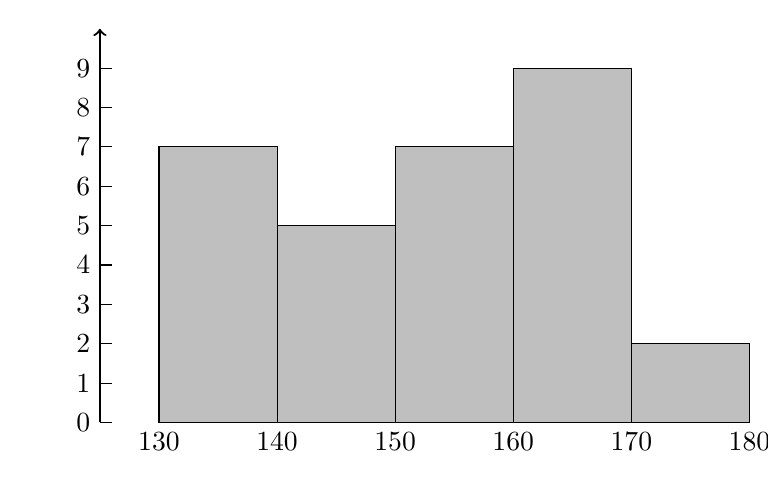
\begin{tikzpicture}[xscale=0.15,yscale=0.5]
      \draw[fill=lightgray] (130,0) rectangle (140,7);
      \draw[fill=lightgray] (140,0) rectangle (150,5);
      \draw[fill=lightgray] (150,0) rectangle (160,7);
      \draw[fill=lightgray] (160,0) rectangle (170,9);
      \draw[fill=lightgray] (170,0) rectangle (180,2);
      % x labels
      \foreach \x in {130, 140, ..., 180} {
        \draw (\x,0) node[anchor=north] {$\x$};
      }
      % y axis
      \draw[thick,->] (125,0) -- (125,10);
      % y labels
      \foreach \y in {0, 1, ..., 9} {
        \draw (125,\y) node[anchor=east] {$\y$} -- (126,\y);
      }
    \end{tikzpicture}
  \end{center}
}
\end{wex}    

With grouped data estimating the measures of central tendency changes
because we've already discarded some information about the original
data set. If all we have to work with is the grouped data, the best we
can do is to assume that values are distributed uniformly in each
range.

TODO Visualise. This leads to the following formulae for mean,
median, mode.

\section{Dispersion}
The central tendency is not the only interesting or useful information
about a data set. The two data sets shown below have the same mean,
but are clearly quite different.

\begin{center}
  FIGURE: two 2d gaussians with equal mean, but different variances.
\end{center}

In this section we will look at measures of dispersion. Dispersion is
a general term for different statistics that describe how values or
distributed around the centre.

\Definition{Range}{The range of a data set is the difference between
  the lowest value and the highest value in the set.}

Range as (a very poor) measure of dispersion. Extremely sensitive to
outliers! Range is inter-percentile range between 0th and 100th
percentile (i.e. min and max).

The most straightforward of the dispersion measures is the range.

\section{Percentiles}

These give a more complete picture. Some measures of central tendency
and dispersion are special cases of percentiles.

There are many percentiles, so we need to specify which one. They are
generally between 0 and 100. We have already seen the one in the
middle, the 50th percentile, the median.

For percentiles: same process as median, just different distances from
the edges.

FIGURE: Show ordered data set again, with 10th percentiles.

0th percentile is the minimum value
100th percentile is the maximum value
50th is value in the middle

\subsection{Quartiles}
Quartiles are special case of percentiles

Interquartile range is a measure of dispersion

Semi-interquartile range is half interquartile range (how silly do
define this).

\subsection{Five number summary}

Visualisation in the box and whisker plot.

-----

Need summary figure of different statistics -- preferably to highlight
how they are the same and how they are different. Classic example:
mode v mean v median.

Need example of something that doesn't follow a bell-shape distribution.

\end{document}
